\subsection{Paket: wrapfigure}

\begin{frame}[fragile]
\frametitle{Abbildungen von Text umfließen lassen}
\framesubtitle{Das Paket \pkg{wrapfig}}

Um Text um Bilder \enquote{herumfließen} zu lassen, benutzen wir das Paket \pkg{wrapfig}.

\begin{codeblock}
\verb|\begin{wrapfigure}|\marg{Ausrichtung}\marg{Breite}\\
\verb|\includegraphics[width=0.5\textwidth]{xkcd.png}|\\
\verb|\end{wrapfigure}|
\end{codeblock}

\begin{itemize}
 \item \textit{Ausrichtung}: Links: \texttt{l}, Rechts: \texttt{r}
 \item \textit{Breite}: Zum Beispiel \texttt{8cm}
 \item Bild nicht rechts/links Ausrichten, da es sonst ggf. in den Text rutscht.
\end{itemize}

\end{frame}

\begin{frame}[fragile]
\frametitle{Abbildungen von Text umfließen lassen}
\begin{wrapfigure}
{l}
{6cm}
\includegraphics[width=0.5\textwidth]{images/xkcd.png}
\end{wrapfigure}
\footnotesize \lipsum[2]
\end{frame}

